\documentclass[a4paper]{article} 
 \usepackage{tikz} 
 \begin{document} 
 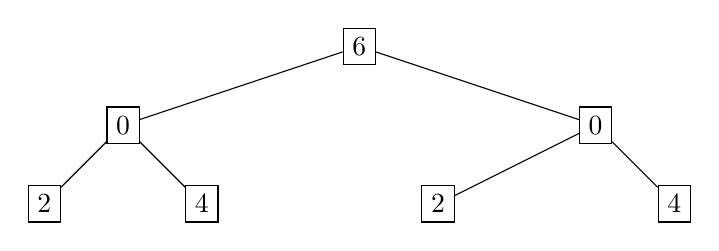
\begin{tikzpicture}
\node[draw] (SZ1) at (5, 1) { 6};
\node[draw] (SZ2) at (2, 0) { 0};
\draw (SZ1) -- (SZ2);
\node[draw] (SZ4) at (1, -1) { 2};
\draw (SZ2) -- (SZ4);
\node[draw] (SZ5) at (3, -1) { 4};
\draw (SZ2) -- (SZ5);
\node[draw] (SZ3) at (8, 0) { 0};
\draw (SZ1) -- (SZ3);
\node[draw] (SZ6) at (6, -1) { 2};
\draw (SZ3) -- (SZ6);
\node[draw] (SZ7) at (9, -1) { 4};
\draw (SZ3) -- (SZ7);

  \end{tikzpicture}
  \end{document} 
